\section{Word Frequency}
\label{appendix2}

The following charts show how often some of the words related to a 'third sex' are used in the Pali canon as well as in the Sanskrit texts. Note that the size of the specific parts of the canon is not taken into account so we have to be careful drawing definite conclusions from these charts, but they do show the relative importance of these words. 

\subsection{Pali canon and commentaries}

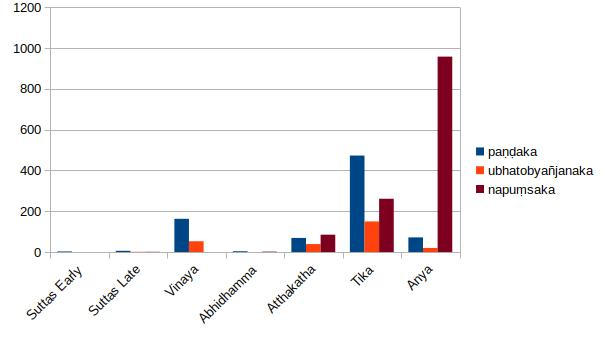
\includegraphics[width=0.7\linewidth]{pali.jpg}
\captionof{figure}{Frequency of words in the Pali canon and commentaries}
\label{pali1}

\subsection{Sanskrit Buddhist and Vedic canon}

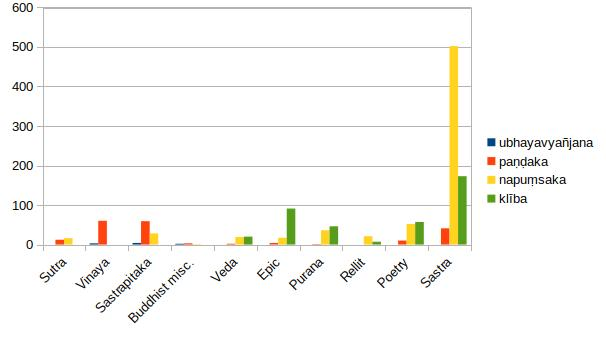
\includegraphics[width=0.7\linewidth]{sanskrit.jpg}
\captionof{figure}{Frequency of words in the Sanskrit Buddhist and Vedic canon}
\label{sanskrit1}

\medskip
It is important to note that unlike the texts in the Pali canon, the search over the Sanskrit text only use the GRETIL database\footnote{\href{http://gretil.sub.uni-goettingen.de/gretil.html}{GRETIL--Göttingen Register of Electronic Texts in Indian Languages.}} and do not comprise the entire Buddhist canon. The Vedic/Brahmanic texts are also included in this chart.
